% Sw practice and experience.

\section{Introduction}
% From ipdps paper

For performance reasons, uniprocessor computers are now being replaced with
small multiprocessors. Moreover, modern processor chips from major processor
manufacturers often contain more than one CPU core, either logically through
Symmetric MultiThreading~\cite{eggers97simultaneous} or physically as a Chip
MultiProcessor~\cite{hammond97singlechip}.  For instance, current Intel
Pentium~4 and Xeon processors contain two logical
processors~\cite{marr02hyperthreading} and several other manufacturers are in
the process of introducing on-chip
multiprocessors~\cite{kahle99power4,spracklen05cmt}. With multiprocessors
becoming prevalent, good operating system support is crucial to benefit from
the increased computing capacity.

% Rewrite???
We are currently working on a project together with a major developer of
industrial systems. The company has over the last 10 years being developing an
operating system kernel for clusters of uniprocessor IA-32 computers. The
operating system has interesting properties such as fault tolerance and high
performance (mainly in terms of throughput). In order to take advantage of new
shared-memory multiprocessors, a multiprocessor version of the kernel is being
developed~\cite{kagstrom05experiences}.  However, we were faced with the
problem that it was very difficult and costly to make the needed modifications
because of the size of the code, the long time during which the code had been
developed (this has led to a code structure which is hard to grasp), and the
intricate nature of operating system kernels.

The situation described above illustrates the fact that making changes to
large software bodies can be very costly and time consuming, and there has
also been a surge of interest in alternative methods lately. For example, as
an alternative to altering operating system code, Arpaci-Dusseau et
al.~\cite{arpacidusseau01information} propose a method where ``gray-box''~
knowledge about algorithms and the behavior of an operating system are used to
acquire control and information over the operating system without explicit
interfaces or operating system modification. There has also been some work
where the kernel is changed to provide quality of service guarantees to large
unmodified applications~\cite{zhang03qos}.

For the kernel of our industrial partner, it turned out that the software
engineering problems when adding multiprocessor support were extremely difficult
and time-consuming to address using a traditional approach. Coupled to the
fact that the target hardware would not scale to a very large number of
processors during the foreseeable future (we expect systems in the range of 2
to 8 processors), this led us to think of another approach. In our approach,
we treat the existing kernel as a black box and build the multiprocessor
adaptations beside it. A custom kernel called \emph{the application kernel},
of which the original kernel is unaware, is constructed to run on the other
processors in the system while the original kernel continues to run on the
boot processor. Applications execute on the other processors while system
calls, page faults, etc., are redirected by the application kernel to the
uniprocessor kernel. We expect the application kernel approach to
substantially lower the development and maintenance costs compared to a
traditional multiprocessor port.

In this paper, we describe the application kernel approach and evaluate an
implementation for the Linux kernel. With this implementation, we demonstrate
that it is possible to implement our approach without changing the kernel
source code and at the same time running unmodified Linux applications. We
evaluate our approach both in terms of performance and implementation
complexity. The evaluation results show that the implementation complexity is
low in terms of lines of code and cyclomatic complexity for functions,
requiring only seven weeks to implement. Performance-wise, our implementation
performance-levels comparable to Linux for compute-bound applications.

The application kernel implementation for Linux is available as free software
licensed under the GNU General Public License (GPL) at
\url{http://www.ipd.bth.se/ska/application_kernel.html}. This paper builds on
our previous work where we implemented the application kernel approach for a
small in-house kernel~\cite{ska2004}.

The rest of the paper is structured as follows. We begin with discussing
related work in Section~\ref{sec:appkern:related_work}. In Section~\ref{sec:appkern:approach}
we describe the ideas behind our approach and Section~\ref{sec:appkern:implementation}
then discusses our implementation for the Linux kernel. We describe our
evaluation framework in Section~\ref{sec:appkern:evaluation_framework}, and then
evaluate the implementation complexity and performance of the application
kernel in Section~\ref{sec:appkern:results}.  Finally, we conclude and discuss future
extensions to the approach in Section~\ref{sec:appkern:conclusion}.


\section{Related Work}
\label{sec:appkern:related_work}
The implementation of a multiprocessor operating system kernel can be
structured in a number of ways.  In this section, we present the traditional
approaches to multiprocessor porting as well as some alternative methods and discuss
their relation to our approach.

\subsection{Monolithic Kernels}
Many multiprocessor operating systems have evolved from monolithic
uniprocessor kernels. These uniprocessor kernels (for example Linux and BSD
UNIX) contain large parts of the actual operating system, making
multiprocessor adaptation a complex task.  In-kernel data structures need to
be protected from concurrent access from multiple processors and this requires
locking. The granularity of the locks, i.e., the scope of the code or data
structures a lock protects, is an important component for the performance and
complexity of the operating system. Early multiprocessor operating systems
often used coarse-grained locking, for example the semaphore-based
multiprocessor version of UNIX described by Bach and
Buroff~\cite{bach84multiprocessor}\label{fix:bach}. These systems employ a
locking scheme where only one processor runs in the kernel (or in a kernel
subsystem) at a time~\cite{schimmel94unix}.  The main advantage with the
coarse-grained method is that most data structures of the kernel can remain
unprotected, and this simplifies the multiprocessor implementation. In the
most extreme case, a single ``giant''~lock protects the entire kernel.

The time spent in waiting for the kernel locks can be substantial for systems
dominated by in-kernel execution, and in many cases actually unnecessary since
the processors might use different paths through the kernel. The obvious
alternative is then to relax the locking scheme and use a more fine grained
locking scheme to allow several processors to execute in the kernel
concurrently.  Fine-grained systems allow for better scalability since
processes can run with less blocking on kernel-access.  However, they also
require more careful implementation, since more places in the kernel must be
locked.  The FreeBSD SMP implementation, which originally used coarse-grained
locking, has shifted toward a fine-grained method~\cite{lehey01freebsd} and
mature UNIX systems such as AIX and Solaris implement multiprocessor support
with fine-grained locking~\cite{clark95symmetric, kleinman92solaris}, as do
current versions of Linux~\cite{love2003linux}.

\subsection{Microkernel-based Systems}
Another approach is to run the operating system on top of a microkernel.
Microkernel-based systems potentially provide better system security by
isolating operating system components and also better portability since much
of the hardware dependencies can be abstracted away by the microkernel. There
are a number of operating systems based on microkernels, e.g.,
L4Linux~\cite{l4linux}, a modified Linux kernel which runs on top of the L4
microkernel~\cite{ukernelconstruction}. The Mach microkernel has been used as
the base for many operating systems, for example DEC~OSF/1~\cite{denham94osf1}
and MkLinux~\cite{mklinux}. Further, QNX~\cite{qnx} is a widely adopted
microkernel-based multiprocessor operating system for real-time tasks.
However, although the microkernel implements lower-level handling in the
system, a ported monolithic kernel still needs to provide locks around
critical areas of the system.

An alternative approach is used in multiserver operating systems~\cite{hurd,
  roscoeroscoestructure}. Multiserver systems organize the system as multiple
separated servers on a microkernel. These servers rely on microkernel
abstractions such as threads and address spaces, which can in principle be
backed by multiple processors transparently to the operating system servers.
However, adapting an existing kernel to run as a multiserver
system~\cite{gefflaut00sawmill, rawson97experience} requires major refactoring
of the kernel. Designing a system from scratch is a major undertaking, so in
most cases it is more feasible to port an existing kernel.


\subsection{Asymmetric Operating Systems}
\label{sec:appkern:related_asymetric}
Like systems which use coarse-grained locking, master-slave systems (refer to
Chapter 9 in~\cite{schimmel94unix}) allow only one processor in the kernel
at a time. The difference is that in master-slave systems, one processor is
dedicated to handling kernel operations (the ``master''~processor) whereas the
other processors (``slaves'') run user-level applications. On system calls and
other operations involving the kernel, master-slave systems divert the
execution to the master processor. Commonly, this is done through splitting
the ready queue into one slave queue and one master queue. Processes are then
enqueued in the master queue on kernel operations, and enqueued in the slave
queue again when the kernel operation finishes. Since all kernel access is
handled by one processor, this method limits throughput for kernel-bound
applications.

The master-slave approach is rarely used in current multiprocessor operating
systems, but was more common in early multiprocessor implementations. For
example, \label{fix:goble}Goble and Marsh~\cite{goble82dualvax} describe an
early tightly coupled VAX multiprocessor system, which was organized as a
master-slave system. The dual VAX system does not split the ready queue, but
instead lets the slave processor scan the ready queue for processes not
executing kernel code. Also, although both processors can be interrupted, all
interrupt handling (except timer interrupts) are done on the master processor.
Our approach is a modern refinement of the master-slave approach, where the
source code of the original system (``master'') remains unchanged.


% From SBAC-PAD paper
An interesting variation of multiprocessor kernels was presented in Steven
Muir's PhD. thesis~\cite{muir01piglet}\label{fix:muir}.
Piglet~\cite{muir01piglet} dedicates the processors to specific operating
system functionality.  Piglet allocates processors to run a Lightweight Device
Kernel (LDK), which normally handles access to hardware devices but can also
perform other tasks. The LDK is not interrupt-driven, but instead polls
devices and message buffers for incoming work. A prototype of Piglet has been
implemented to run beside Linux 2.0.30, where the network subsystem (including
device handling) has been off-loaded to the LDK, and the Linux kernel and
user-space processes communicate through lock-free message buffers with the
LDK. A similar approach has also been used to offload the TCP/IP stack
recently~\cite{regnier2004tcp}. These approaches are beneficial if
I/O-handling dominates the OS workload, whereas it is a disadvantage in
systems with much computational work when the processors would serve better as
computational processors. It can also require substantial modification of the
original kernel, including a full multiprocessor adaption when more than one
processor is running applications.

\subsection{Cluster-based Approaches}
% Make this sort of cluster-dependent
Several approaches based on virtualized clusters have also been presented. One
example is the Adeos Nanokernel~\cite{yaghmour2002} where a multiprocessor
acts as a cluster with each processor running a modified version of the Linux
kernel. The kernels cooperate in a virtual high-speed and low-latency network.
The Linux kernel in turn runs on top of a bare-bones kernel (the Adeos
nanokernel) and most features of Linux have been kept unchanged, including
scheduling, virtual memory, etc. This approach has also been used in
Xen~\cite{barham03xen}\label{fix:xen}, which virtualizes Linux or NetBSD
systems.

Another cluster-based method is Cellular Disco~\cite{govil99cellular}, where
virtualization is used to partition a large NUMA multiprocessor into a virtual
cluster which also provides fault-containment between the virtualized
operating systems. The virtualized systems provide characteristics similar to
our approach in that they avoid the complexity issues associated with a
traditional parallelization approach. However, they also require a different
programming model than single-computer systems for parallel applications.
Cluster-based approaches are also best suited for large-scale systems where
scalability and fault tolerance are hard to achieve using traditional
approaches.

MOSIX~\cite{mosix} is a single system image distributed system which redirects
system calls to the ``unique home node''~of the process, thereby utilizing the
central idea behind master-slave systems. MOSIX can distribute unmodified
Linux applications throughout a cluster of asymmetric hardware. MOSIX is
similar to our approach in that it redirects system calls, but has a different
goal (providing a single-system image distributed system).

\section{The Application Kernel Approach}

\label{sec:appkern:approach}
All of the approaches presented in the last section require, to various
degrees, extensive knowledge and modifications of the original kernel. We
therefore suggest a different approach, the \emph{application kernel
  approach}, which allows adding multiprocessor support with minimal effort
and only basic knowledge about the original kernel. In this section we
describe the general ideas behind the application kernel approach and an
overview of how it works.

\subsection{Terminology and Assumptions}
Throughout the paper, we assume that the implementation platform is the Intel
IA-32 although the approach is applicable to other architectures as well. We
will follow the Intel terminology when describing processors, i.e., the
processor booting the computer will be called the \emph{bootstrap processor}
while the other processors in the system are called \emph{application
  processors}.

Also, we use a similar naming scheme for the two kernels: the original
uniprocessor kernel is called the \emph{bootstrap kernel}, i.e., the Linux
kernel in the implementation described in this paper, whereas the second
kernel is called the \emph{application kernel}.  Further, in order to not
complicate the presentation, we will assume single-threaded processes in the
discussion, although multi-threaded processes are also supported using the
same technique.

\subsection{Overview}
The basic idea in our approach is to run the original uniprocessor kernel
\emph{as it is} on the bootstrap processor while all other processors run the
application kernel. Applications execute on both kernels, with the application
kernel handling the user-level part and the bootstrap kernel handling
kernel-level operations.  One way of describing the overall approach is that
the part of the application that needs to communicate with the kernel is
executed on a single bootstrap processor while the user-level part of the
program is distributed among the other processors in the system, i.e., similar
to master-slave kernels.

\begin{figure}
  \begin{center}
    \epsfig{width=0.6\linewidth, file=figures/linux-appkern/general_structure}
  \end{center}
  \caption{Overview of the application kernel approach.}
  \label{fig:approach}
\end{figure}

Figure~\ref{fig:approach} shows an overview of the application kernel
approach. The upper boxes represent user processes and the lower shows the
bootstrap kernel and the application kernel. Each process has two threads, a
\emph{bootstrap thread} and an \emph{application thread}. The bootstrap thread
executes on the bootstrap kernel, i.e., Linux, while the application threads
are handled by the application kernel. An application thread runs the actual
program code whereas the bootstrap thread serves as a proxy\label{fix:relay}
forwarding kernel calls to the bootstrap kernel. Note that the application
kernel and the bootstrap kernel use unique interrupt and trap handlers to
enable the application kernel to catch traps and faults caused by the
application.

The two threads in the process' communicate through a shared area in the
process address space. The bootstrap monitors the shared area to detect new
system calls etc. Applications run as before, except when performing
operations involving the kernel. On such events, the application thread traps
into the application kernel, which then enters a message in the communication
area. The actual event will be handled at a later stage by the bootstrap
thread, which performs the corresponding operation. We will describe trap
handling in detail in Section~\ref{sec:appkern:trap_handling}.

With the application kernel approach, we can add multiprocessor support to an
existing operating system without neither doing modifications to the original
operating system kernel, nor do we have to do any changes to the applications
(not even recompiling them). There are a few special cases that might require
kernel source changes, but those were not needed for our research prototype.
Section~\ref{sec:appkern:implementation_paging} describes these special cases.

Compared to the other porting methods, our approach tries to minimize the
effort needed to implement a multiprocessor port of a uniprocessor operating
system.  The focus is therefore different from traditional porting methods.
Master-slave kernels, which are arguably most similar to our approach, place
most of the additional complexity in the original kernel whereas we put it
into two separate entities (the application kernel and the bootstrap thread).
In a sense, our approach can be seen as a more general revitalization of the
master-slave idea. The Cache Kernel~\cite{greenwald96synergy,
  cheriton94caching} employs a scheme similar to ours on redirecting system
calls and page faults, but requires a complete reimplementation of the
original kernel to adapt it to the cache kernel. We can also compare it to the
MOSIX system~\cite{mosix} which also redirects system calls, although MOSIX is
used in a cluster context and has different goals then the application kernel.

\subsection{Hardware and Software Requirements}
The application kernel approach places some restrictions (often easy to
fulfill) on the processor architecture and the bootstrap kernel. The
architecture must support at least the following:

\begin{enumerate}
\item Binding of external interrupts to a specific processor and at the same
  time allow CPU-local timer interrupts.
\item Retrieving the physical page table address of the currently running
  process.
\item Interrupt and trap handlers must be CPU-local.
\end{enumerate}

The first requirement must be fulfilled since only the bootstrap kernel
handles all external interrupts except for timer interrupts. Timer interrupts
need to be CPU-local for scheduling to take place on the application kernel.
On the IA-32 this is possible to implement with the APIC (Advanced
Programmable Interrupt Controller), which has a per-processor timer.
\label{fix:local_timer}MIPS uses a timer in the coprocessor 0 on the processor
chip~\cite{mips01programmers} and PowerPC has a decrementer
register~\cite{ppcrefman} which can be used to issue interrupts.  The
interrupt \emph{handlers} must be private for different processors, which is
directly possible on IA-32 processors through the Interrupt Descriptor Table,
IDT. For architectures where the interrupt handlers reside on fixed addresses,
e.g., MIPS, instrumentation of the interrupt handlers are needed.

Our approach also places two requirements on the bootstrap kernel. First, it
must be possible to extend the kernel with code running in supervisor mode.
This requirement is satisfied in most operating systems, e.g., through
loadable modules in Linux. Second, the bootstrap kernel must not change or
remove any page mappings from the application kernel. The application kernel
memory needs to be mapped to physical memory at all times, since revoking a
page and handing it out to a process (or another location in the kernel) would
cause the application kernel to overwrite data for the bootstrap kernel or
processes.



\subsection{Application Kernel Interaction}
\label{sec:appkern:trap_handling}

Figure~\ref{fig:trap} shows how the kernel interaction works in the application
kernel approach. Kernel interaction requires 8 steps, which are illustrated in
the Figure. In the discussion, we assume that the operation is a system call,
although page faults and other operations are handled in the same way.

\begin{figure}
  \begin{center}
    \epsfig{width=0.6\linewidth, file=figures/linux-appkern/trap}
  \end{center}
  \caption[System call and trap handling]{System call/trap handling in the application kernel approach}
  \label{fig:trap}
\end{figure}

\begin{enumerate}
\item The application (i.e., the application thread running on one of the
  application processors) issues a system call and traps down to the
  application kernel. This is handled by the CPU-local trap vector.

\item The application kernel enters information about the call into the shared
  area, and thereafter schedules another thread for execution.
\item At a later point, the bootstrap thread wakes up and finds a message in
  the shared area.
\item The bootstrap thread then parses the message and performs the
  corresponding operation (i.e., issuing the same system call in this case).
\item The bootstrap kernel will thereafter handle the system call from the bootstrap
  thread and  return control to the bootstrap thread.
\item After this, the bootstrap thread must tell the application kernel that
  the application thread can be scheduled again. Since the application kernel
  runs as a loadable module within the bootstrap kernel, it must do this
  through the driver interface of the bootstrap kernel, issuing the
  application kernel \textbf{apkern\_activate\_thread} call.
\item The application kernel driver, running on the bootstrap processor,
  enters the application thread into the ready queue again.
\item Finally, the application thread is scheduled at a later point in time on
  one of the application processors.
\end{enumerate}

The \texttt{clone} and \texttt{fork} system calls are handled slightly
different then other calls, and are described in detail in
Section~\ref{sec:appkern:clone}.  Further, the \texttt{exit} system call and
exceptions that cause process termination (for example illegal instructions)
are different than page faults and other system calls. This is because the
bootstrap kernel is unaware of the application thread and will terminate the
process without notifying the application kernel. If this is not handled, the
application kernel will later schedule a thread which runs in a non-existing
address space. For this case, step 2 of the algorithm above is modified to
clean up the application thread (i.e., free the memory used by the thread
control block and remove the thread from any lists or queues).

Another special case is when the information flows the opposite way, i.e.,
when the kernel asynchronously activates a process (for instance in response
to a signal in Linux). In this case, the handler in the bootstrap thread will
issue the \textbf{apkern\_activate\_thread} call directly, passing information
about the operation through the shared area. The application kernel will then
issue the same signal to the application thread, activating it asynchronously.
\label{fix:signal_handlers}Our current implementation does not support
asynchronous notifications, but it would be achieved by registering signal
handlers during the bootstrap thread startup phase.


\subsection{Exported Application Programming Interface}
The application kernel API is only available via driver calls to the bootstrap
kernel. There is no way to call the application kernel directly via system
calls in the application thread since the trap handling matches that of the
bootstrap kernel and only forwards the events through the shared area. A
straightforward way of allowing direct calls to the application kernel would
be to use a different trap vector\label{fix:trap_vector} than the Linux
standard, which could be used e.g., to control application kernel scheduling
from applications. The exported interface consists of six calls:

\begin{itemize}
\item \textbf{apkern\_init}: This routine is called once on system startup,
  typically when the application kernel device driver is loaded. It performs
  the following tasks:
  \begin{itemize}
  \item It initializes data structures in the application kernel, for example the
    ready-queue structure and the thread lookup table.
  \item It starts the application processors in the system. On startup, each
    processor will initialize the interrupt vector to support system calls and
    exceptions. The processor will also enable paging and enter the idle
    thread waiting for timer interrupts.
  \end{itemize}
\item \textbf{apkern\_thread\_create}: This function is called from the
  bootstrap thread when the process is started. The function creates a new
  thread on the application kernel. The thread does not enter the ready queue
  until the \textbf{apkern\_thread\_start} call is invoked.

\item \textbf{apkern\_thread\_ex\_regs}: Sometimes it is necessary to update
  the register contents of a thread (for example copying the register contents
  from parent to child when forking a process), and the application kernel
  therefore has a call to ``exchange'' the register contents of a thread.

\item \textbf{apkern\_thread\_get\_regs}: This function returns in the current
  register context of a thread (also used with fork).

\item \textbf{apkern\_thread\_start}: Place a thread in the ready queue.

\item \textbf{apkern\_thread\_activate}: Thread activation is performed when
  the bootstrap thread returns, e.g., from a system call, to wake up the
  application thread again. The call will enter the application thread back
  into the ready queue and change its state from \emph{blocked} to
  \emph{ready}.
\end{itemize}



\section{Implementation}

\label{sec:appkern:implementation}

We implemented the application kernel as a loadable kernel module for Linux.
The module can be loaded at any time, i.e., the application kernel does not
need to be started during boot but can be added when it is needed. Since
modules can be loaded on demand, the application kernel can also be started
when the first process uses it. It is further not necessary to recompile
applications to run on the application kernel, and applications running on the
application kernel can coexist seamlessly with applications running only on
the bootstrap processor.

\label{fix:shared_area}The layout of the shared memory area for the Linux
implementation is shown in Figure~\ref{fig:shared_area}. The shared area data
type, \texttt{apkern\_comm\_entry\_t} has a union with the different types of
messages, with page faults and system calls shown in the figure and a variable
(\texttt{bootstrap\_has\_msg}) which is used by the application kernel to
signal to the bootstrap thread. There is always a one to one mapping between
application threads and bootstrap threads, i.e., multithreaded processes will
have several bootstrap thread. The bootstrap thread does not respond to system
calls etc., through the shared area, but invokes the application kernel driver
instead. Since the shared area is a one-way communication channel, it needs no
explicit protection.

\begin{figure}
  \footnotesize
  \begin{verbatim}
typedef struct {
  volatile bool_t bootstrap_has_msg;
  volatile apkern_comm_nr_t nr;
  volatile addr_t pc;

  union {
    struct {
      volatile addr_t addr;
      volatile bool_t write;
    } PACKED pagefault;

    struct {
      volatile uint_t nr;
      volatile uint_t arg1;
      ...
      volatile uint_t arg6;
      volatile uint_t ret;
    } PACKED syscall;
    ...
  } u;
} apkern_comm_entry_t;
  \end{verbatim}
  \caption{Shared area layout}
  \label{fig:shared_area}
\end{figure}

The application kernel is initialized, i.e., processors are booted etc., when
the kernel module is loaded. The application kernel is thereafter accessible
through a normal Linux device file, and a process that wants to run on the
application kernel opens the device file on startup and closes it when it
exits (this can be done automatically and is described in
\label{fix:forward_ref}Section~\ref{sec:appkern:running_applications}).  All interactions with the
application kernel, apart from \texttt{open} and \texttt{close}, are done
using \texttt{ioctl} calls, through which the exported interface is available.

\label{fix:device_driver}Figure~\ref{fig:driver_structure} illustrates the
application kernel driver (a char-type device) structure and an
\textbf{apkern\_activate\_thread} call. The call from the bootstrap thread
enters through the Linux system call handler which forwards it to the
\texttt{ioctl} entry point for the device driver. The \texttt{ioctl} handler
in turn updates the thread control block for the activated thread, locks the
application kernel ready queue, and enters the thread control block into the
ready queue. In the rest of this section, we will discuss details related to
paging, forking and application startup from the Linux implementation of the
application kernel.


\begin{figure}
  \begin{center}
    \epsfig{width=0.7\linewidth, file=figures/linux-appkern/driver_structure}
  \end{center}
  \caption{Application kernel device driver structure}
  \label{fig:driver_structure}
\end{figure}


\subsection{Paging}
% Paging
\label{sec:appkern:implementation_paging}

All page faults are handled in the bootstrap thread by setting the stack
pointer to the address of the page fault and touching that memory area.
Although this seems like an unnecessary step instead of just accessing the
memory directly, it is needed as a workaround since Linux terminates the
program if stack access is done below the current stack pointer.

The paging implementation also illustrates the one case where the application
kernel approach might require kernel modifications. The problem (which is
general and affects other approaches as well) occurs in multi-threaded
processes on page table updates, when the translation lookaside buffer (TLB)
contents for different processors running in the same address space will be
inconsistent\footnote{On architectures with tagged TLBs, e.g., MIPS, this
  could occur even in single-threaded processes since the TLB is not
  necessarily flushed on page table switches.}. For example, if processor 0
and 1 execute threads in the same address space, and processor 0 revokes a
page mapping, the TLB of processor 1 will contain an incorrect cached
translation. To solve this, an inter-processor interrupt is invoked to
invalidate the TLB of the other processors, which requires changes to the page
fault handling code. In our prototype, we ran without disk swap and the
inter-processor interrupts are therefore not needed and have not been
implemented.

% clone
\subsection{\texttt{clone}/\texttt{fork} System Calls}
\label{sec:appkern:clone}
The Linux \texttt{clone} and \texttt{fork} system calls require special
handling in the application kernel. Both calls start a new process which
inherits the context of the invoking thread. The difference is that
\texttt{clone} allows for sharing the address space with the parent (creating
a new thread), while \texttt{fork} always separate the address spaces
(creating a new process).  \texttt{clone} also requires the invoker to specify
a callback function that will be executed by the cloned thread.  In Linux,
\texttt{fork} is simply a special case of \texttt{clone},
\label{fix:clone}although the implementation of \texttt{fork} predates
\texttt{clone}.

We illustrate the steps needed in a \texttt{clone} or \texttt{fork} call in
Figure~\ref{fig:clone}. If we would just issue the system call directly, the
bootstrap thread would run the cloned thread itself. Therefore we first clone
the bootstrap thread, then let the cloned bootstrap thread create a new
application kernel thread (i.e., handling the original clone), and finally
enters a loop waiting for messages from the application kernel. This
effectively splits the \texttt{clone} call in two, creating a new thread pair.
The \texttt{fork} call works the same way, but has different return semantics,
i.e., it returns ``twice''~instead of using a callback.

\begin{figure}
  \begin{center}
    \epsfig{width=0.7\linewidth, file=figures/linux-appkern/fork}
  \end{center}
  \caption{Handling of the \texttt{clone} system call}
  \label{fig:clone}
\end{figure}

\subsection{Running Applications}
\label{sec:appkern:running_applications}
Our implementation allows running dynamically linked applications directly,
without modifying or even recompiling them. It is also possible to run a mixed
system, with some applications running on the application kernel whereas
others are tied to the bootstrap processor.

We achieve this by applying some knowledge about application startup under
Linux. In Linux, applications are started by a short assembly stub which in
turn calls \texttt{\_\_libc\_start\_main}. This function, provided by GNU
libc, starts the \texttt{main} function.  The \texttt{\_\_libc\_start\_main}
function is dynamically linked into the executable and can therefore be
overridden. We override \texttt{\_\_libc\_start\_main} with the startup
routine for the application kernel, which can be done as long as the
application is dynamically linked against libc. To run a process on the
application kernel, we simply set the \texttt{LD\_PRELOAD} environment
variable to preload a library with the bootstrap thread implementation.

\begin{figure}
  \begin{center}
    \epsfig{width=0.7\linewidth, file=figures/linux-appkern/app_startup}
  \end{center}
  \caption[Application startup]{Application startup. The dashed lines shows the original execution
    while the solid lines show the overridden execution path.}
  \label{fig:start_main_override}
\end{figure}

The overriding process is illustrated in Figure~\ref{fig:start_main_override}.
The overridden \texttt{\_\_libc\_start\_main} will just invoke the original
\texttt{\_\_libc\_start\_main}, but with \texttt{apkern\_thread} instead of
\texttt{main} as starting function. This function in turn will either,
depending on if the \texttt{NOAPPKERN} environment variable is set, invoke the
original \texttt{main} and thereby bypassing the application kernel, or start
the bootstrap thread.


\section{Experimental Setup and Methodology}
\label{sec:appkern:evaluation_framework}
We have conducted an evaluation of the application kernel approach where we
evaluate both latency and throughput. First, we measure single-process
performance in order to estimate the extra latency caused by the application
kernel. Second, we measure scalability of multiprogramming and parallel
benchmarks. In the evaluation, we use standard UNIX tools, the
SPLASH~2~\cite{cameron95splash} benchmarks and the SPEC
CPU2000~\cite{spec2000} benchmark suite. Further, we have also evaluated the
implementation size and complexity of our approach, which was performed by
counting the physical lines of code in the application kernel and calculating
the McCabe cyclomatic complexity~\cite{fenton98swmetrics} which gives the
number of independent code paths through a function. The code lines were counted
with the sloccount tool~\cite{sloccount} by David A. Wheeler and the cyclomatic
complexity was measured by the pmccabe tool by Paul Bame~\cite{pmccabe}.

\subsection{Evaluation Environment}

We performed our performance evaluation using the Simics full system
simulator~\cite{simics} and real hardware. We setup Simics to simulate a
complete IA-32 system with 1 to 8 processors. Our hardware is a 200MHz dual
Pentium Pro with 8KB first-level instruction and data caches, and a 256KB
per-processor L2 cache. The Simics simulator allows us to use unmodified hard
disk images, containing the complete operating system.  Compared to real
hardware, our simulated setup does not simulate caches in the system, and some
other performance issues relevant in multiprocessor
systems~\cite{gamsa95performance}, such as costs associated with data
alignment, cross-processor cache access etc., are not accounted for in our
simulations. Our prototype also has known performance issues, e.g., we have
not optimized the memory layout for efficient use of the cache. However, the
fundamental limitation of the application kernel approach is that the
bootstrap thread at some point will be a scalability bottleneck. We believe
that the simulated measurements give a good indication of when this bottleneck
is reached for various usage patterns.

\label{fix:hardware}The execution on hardware serves to validate the correctness of our
implementation in a real setting, and is also used to establish the latency
for kernel operations with the application kernel. We successfully ran all the
benchmarks on our hardware as well as on the simulated system.

We benchmarked uniprocessor Linux with the application kernel module against
multiprocessor Linux, running the 2.4.26 version of the kernel, henceforth
referred to as SMP Linux. Our experiments report the time required to execute the
benchmarks in terms of clock cycles on the bootstrap processor. Our system was
a minimal Debian GNU/Linux 3.1 (``Sarge'')-based distribution, which ran
nothing but the benchmark applications.

\begin{table}
  \caption{The benchmarks used in the performance evaluation}
  \begin{center}
    \begin{small}
      \label{tab:benchmarks}
      \begin{tabular}{p{2.6cm}|l|p{4.2cm}}
        Benchmark & Command & Description \\
        \hline
        \multicolumn{3}{l}{} \\
        \multicolumn{3}{l}{\textbf{Single-process benchmarks}} \\
        \hline
        find & \texttt{find /} & List all files in the system (13,946 files and directories) \\
        \hline
        SPEC2000 gzip & \texttt{164.gzip lgred.log} & Compression of a logfile,
        computationally intensive. \\
        \hline
        SPEC2000 gcc & \texttt{176.gcc smred.c-iterate.i} & SPEC 2000 C-compiler. \\
        & \texttt{-o a.s} \\
        \hline
        \multicolumn{3}{l}{} \\
        \multicolumn{3}{l}{\textbf{Parallel benchmarks}} \\
        \hline
        SPLASH2 RADIX & \texttt{RADIX -n 8000000 -p8} & Sort an array with radix
        sort, 8 threads.\\
        \hline
        SPLASH2 FFT & \texttt{FFT -m20 -p8} & Fourier transform, 8 threads. \\
        \hline
        SPLASH2 LU (non-contiguous) & \texttt{LU -p 8 -b 16 -n 512} & Matrix
        factorization, 8 threads. \\
        \hline
        \multicolumn{3}{l}{} \\
        \multicolumn{3}{l}{\textbf{Multiprogramming benchmarks}} \\
        \hline
        176.gcc & \texttt{176.gcc smred.c-iterate.i} & SPEC2000 C-compiler \\
        & \texttt{-o a.s} \\
        \hline
        find & \texttt{find /} & List all files in the system (13,946 files and
        directories). \\
        \hline
        grep & \texttt{grep "linux" System.map} & Search for an expression
        in a file. System.map has 150,000 lines. \\
        \hline
        find and grep & \texttt{find / | grep "data"} & List all files in the
        system and search for a string in the results.\\
        \hline
        SPLASH2 FFT & \texttt{FFT -m10 -p8} & Fourier transform, 8 threads. \\
        \hline
        SPLASH2 LU & \texttt{LU -p 8 -b 16 -n 512} &
        Matrix factorization, 8 threads. \\
      \end{tabular}
    \end{small}
  \end{center}
\end{table}

\subsection{Benchmarks}
For the performance evaluation, we conducted three types of performance
measurements. First, we ran a number of single-process benchmarks to evaluate
the overhead caused by the system call forwarding used by the application
kernel approach. These benchmarks run one single-threaded process at a time
and should therefore be unaffected by the number of processors. Second, we
also ran a set of multithreaded parallel applications, which shows the
scalability of compute-bound applications. Third, we also evaluated a
multiprogramming workload. In the multiprogramming benchmark, we ran a set of
programs concurrently and measured the duration until the last program
finished. This benchmark should be characteristic of a loaded multi-user
system.

The programs we used are a subset of the SPEC CPU2000 benchmarks, a subset of
the Stanford SPLASH 2 benchmarks, and a set of standard UNIX tools. For SPEC
CPU2000, we used the Minnespec reduced workloads~\cite{minnespec} to provide
reasonable execution times in our simulated environment. The SPLASH 2
benchmarks were compiled with a macro package which uses \texttt{clone} for
the threading implementation and pthread primitives for mutual exclusion. The
SPLASH SPEC benchmarks were compiled with GCC version 3.3.4 (with optimization
-O2) and the UNIX applications were unmodified Debian binaries. The benchmark
applications are summarized in Table~\ref{tab:benchmarks}.

\section{Experimental Results}
\label{sec:appkern:results}
In this Section, we describe the results obtained from our measurements.
Table~\ref{tab:single_process} and \ref{tab:parallel} show the speedup vs.
uniprocessor Linux for SMP Linux and the application kernel. For the parallel
and multiprogramming benchmarks, the speedup is also shown in
Figure~\ref{fig:parallel}. The results from the \texttt{getpid} evaluation is
shown in Table~\ref{tab:getpid}.


\subsection{Performance Evaluation}
\begin{table}
  \caption{\texttt{getpid} latency in Linux and the application kernel}
  \begin{center}
    \label{tab:getpid}
    \begin{small}
      \begin{tabular}{l|rr}
        & Linux & Application Kernel \\
        \hline
        PPro 200MHz & 970 & 5,700 \\
        Simics & 74 & 860 \\
      \end{tabular}
    \end{small}
  \end{center}
\end{table}

\label{fix:lmbench}On our hardware, issuing a \texttt{getpid} call takes
around 970 cycles in Linux on average (the value fluctuates between 850 and
1,100 cycles) whereas the same call requires around 5,700 cycles with the
application kernel as shown in Table~\ref{tab:getpid}.  In Simics, the cost of
performing a \texttt{getpid} call is 74 cycles in Linux and around 860 cycles
with the application kernel. Since \texttt{getpid} performs very little
in-kernel work, the cost for Linux is dominated by the two privilege level
switches (user mode to kernel and back). For the application kernel, there are
five privilege level switches (see Figure~\ref{fig:trap}). First, the
application thread traps down into the application kernel, which updates the
shared area. The bootstrap thread thereafter performs another trap for the
actual call and upon return invokes the application kernel driver through an
\texttt{ioctl} call, i.e., performing another three privilege level switches.
Finally, the application thread is scheduled again, performing the fifth
privilege level switch. In our simulated system, each instruction executes in
one cycle and there is no additional penalty for changing privilege mode and
therefore the \texttt{getpid} cost is dominated by the number of executed
instructions.  This explains why the application kernel overhead is
proportionally larger in the simulated system than on real hardware.

\begin{table*}
  \caption[Single-process speedup]{Speedup for the single-process benchmarks.}
  \begin{center}
    \label{tab:single_process}
    \begin{footnotesize}
      \begin{tabular}{r|rr|rr|rr}
        \hline
        & \multicolumn{6}{c}{Speedup vs. uniprocessor Linux} \\
        & \multicolumn{2}{c}{Find} & \multicolumn{2}{c}{176.gcc} & \multicolumn{2}{c}{164.gzip} \\
        CPUs & Linux & Appkern  & Linux & Appkern  & Linux & Appkern \\
        \hline
        % Find                    176.gcc           164.gzip
2 & 0.9803 & 0.7844 & 1.0015 & 0.8976 & 1.0008 & 0.9461 \\
3 & 0.9795 & 0.8284 & 1.0033 & 0.9125 & 1.0012 & 0.9461 \\
4 & 0.9807 & 0.8641 & 1.0047 & 0.9218 & 1.0014 & 0.9462 \\
5 & 0.9804 & 0.8690 & 1.0053 & 0.9230 & 1.0016 & 0.9462 \\
6 & 0.9800 & 0.8748 & 1.0047 & 0.9244 & 1.0016 & 0.9462 \\
7 & 0.9795 & 0.8784 & 1.0050 & 0.9252 & 1.0017 & 0.9462 \\
8 & 0.9776 & 0.8831 & 1.0055 & 0.9260 & 1.0017 & 0.9462 \\

        \hline
      \end{tabular}
    \end{footnotesize}
  \end{center}
\end{table*}

In the computationally intensive single-process \texttt{gcc} and \texttt{gzip}
benchmarks from SPEC CPU2000, the application kernel performs almost on-par
with SMP Linux (the difference is between 5 and 10\%) as shown in
Table~\ref{tab:single_process}.  Further, we can also see that as more
processors are added, the gap decreases because there is a higher probability
of a processor being free to schedule the thread when the bootstrap thread has
handled the call.

A weak spot for the application kernel shows in the filesystem-intensive
\texttt{find} benchmark. Here, the overhead associated with forwarding system
calls prohibit the application kernel to reach SMP Linux performance levels.
However, since application kernel applications can coexist seamlessly with
applications tied to the bootstrap kernel, it is easy to schedule these
applications on the bootstrap kernel.

\begin{table*}
  \caption[Parallel and multiprogramming speedup]{Speedup for the parallel and multiprogramming benchmarks.}
  \begin{center}
    \label{tab:parallel}
    \begin{footnotesize}
      \begin{tabular}{r|rr|rr|rr|rr}
        \hline
        & \multicolumn{6}{c}{Speedup vs uniprocessor Linux} \\
        & \multicolumn{2}{c}{RADIX} & \multicolumn{2}{c}{FFT} & \multicolumn{2}{c}{LU} & \multicolumn{2}{c}{Multiprogramming} \\
        CPUs & Linux & Appkern  & Linux & Appkern  & Linux & Appkern & Linux & Appkern\\
        \hline
        2 & 2.0433 & 1.0834& 1.6916 & 1.0401 & 1.9217 & 1.2662 & 1.5049 & 0.9705 \\
3 & 3.3758 & 2.5174& 2.2930 & 1.8654 & 2.9430 & 2.0795 & 1.6627 & 1.1375 \\
4 & 4.0885 & 3.7227& 2.5090 & 2.3235 & 3.5053 & 2.9941 & 1.6850 & 1.1779 \\
5 & 5.1898 & 4.8200& 2.8456 & 2.6323 & 4.0857 & 3.8009 & 1.6782 & 1.1878 \\
6 & 5.9562 & 5.5736& 2.9927 & 2.8626 & 4.7706 & 5.0445 & 1.6845 & 1.1962 \\
7 & 6.9355 & 6.1934& 3.1732 & 3.0188 & 5.3277 & 5.1628 & 1.6803 & 1.2059 \\
8 & 8.0009 & 6.0924& 3.3272 & 3.0745 & 6.0084 &        & 1.6839 &        \\

        \hline
      \end{tabular}
    \end{footnotesize}
  \end{center}
\end{table*}

The selected computationally intensive parallel benchmarks from the Stanford
SPLASH 2 suite exhibit good scalability both in SMP Linux and for the
application kernel (see Table~\ref{tab:parallel} and
Figure~\ref{fig:parallel}). The results for the application kernel are close
to those for SMP Linux, especially considering that the application kernel
excludes one of the processors (the bootstrap processor) for computation. This
shows that the application kernel is a feasible approach for computationally
intensive applications, where the kernel interaction is limited.

\begin{figure*}
  \caption[Speedup vs uniprocessor Linux]{Speedup for the parallel and multiprogramming benchmarks vs.
    uniprocessor Linux.}
  \begin{center}
    \begin{small}
      \begin{tabular}{cc}
        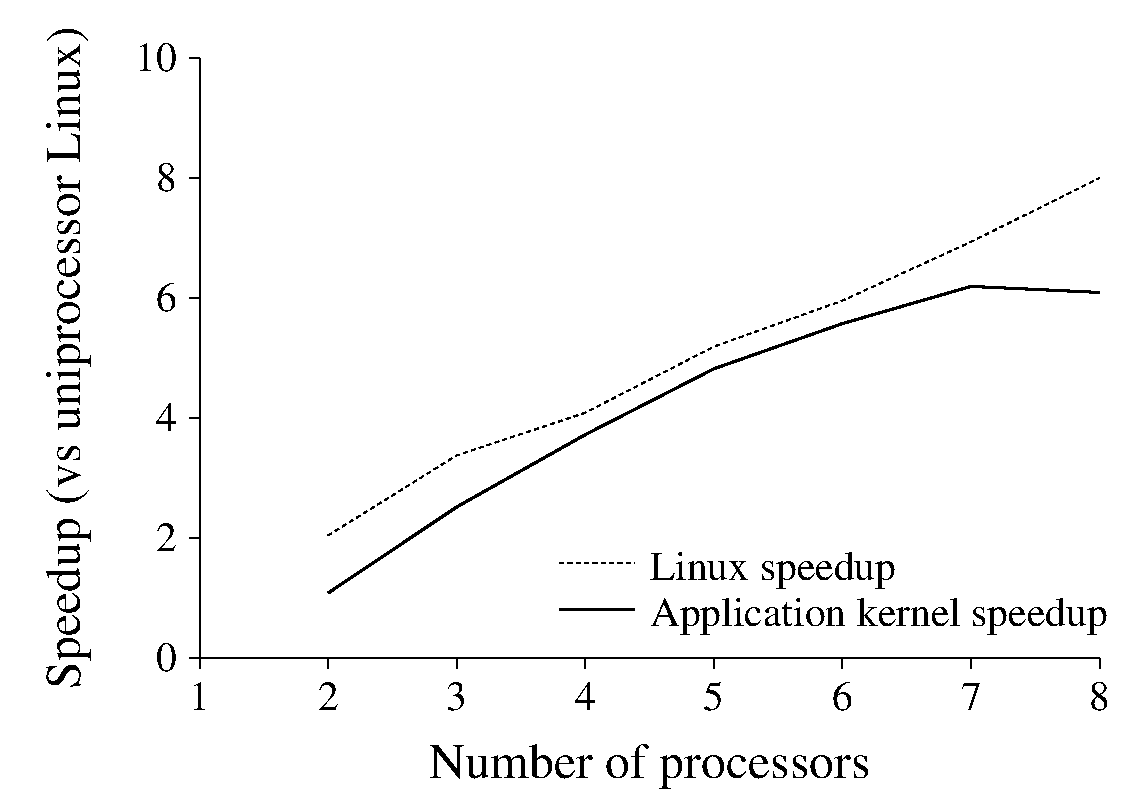
\epsfig{width=0.44\linewidth, file=./data/linux-appkern/RADIX_p8}\hspace{1.0cm} & 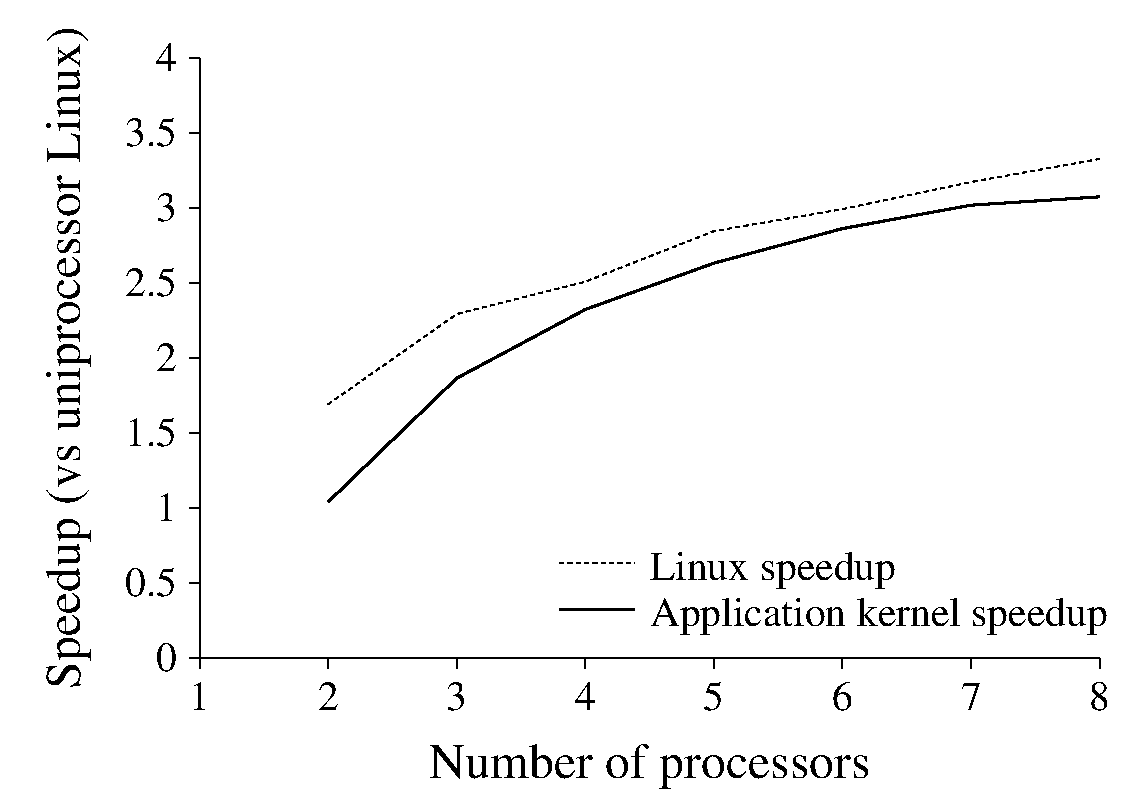
\epsfig{width=0.44\linewidth, file=./data/linux-appkern/FFT_p8}\\
        RADIX & FFT \\
        \vspace{0.1cm}
        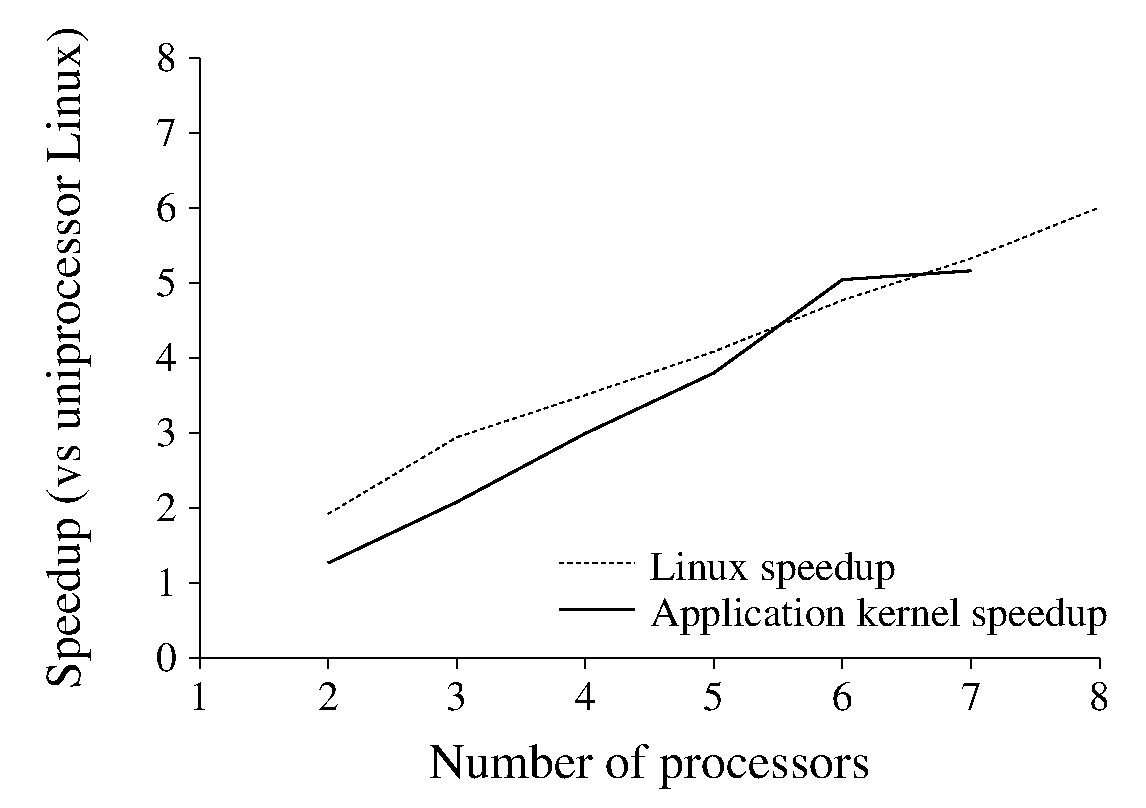
\epsfig{width=0.44\linewidth, file=./data/linux-appkern/lu_non_cont}\hspace{1.0cm} & 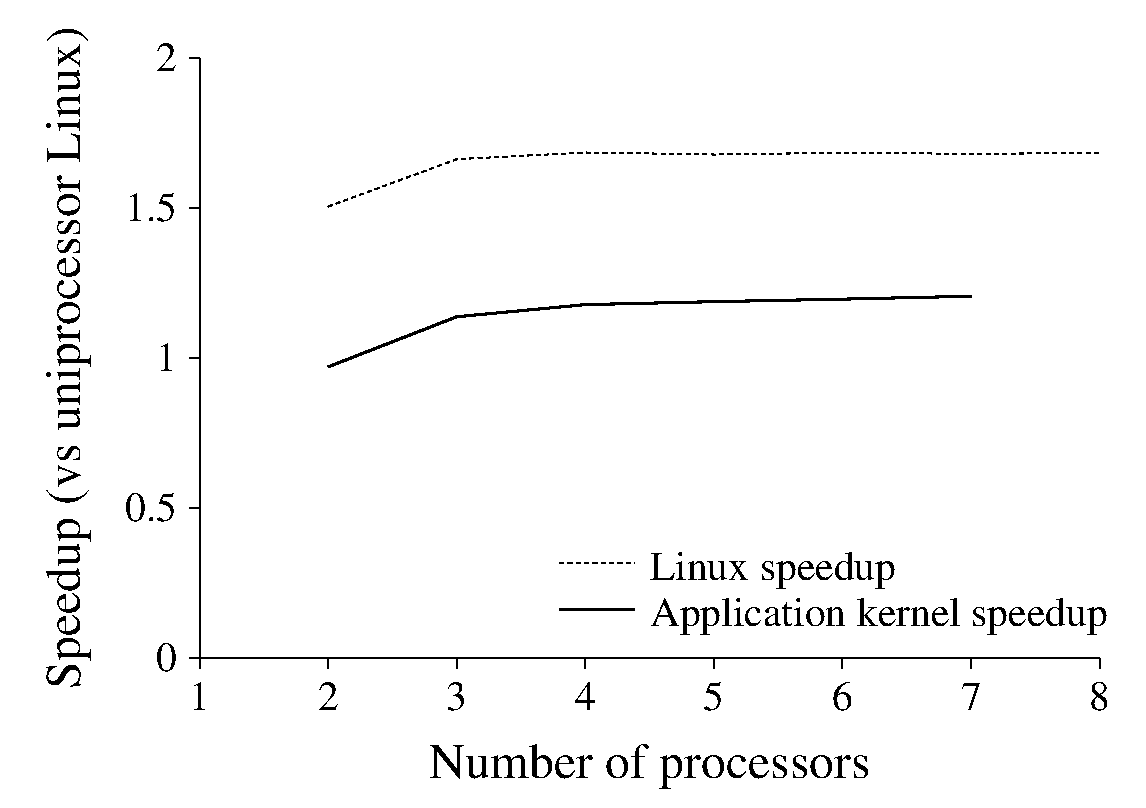
\epsfig{width=0.44\linewidth, file=./data/linux-appkern/multiprogramming}\\
        LU & Multiprogramming \\
      \end{tabular}
    \end{small}
    \end{center}
  \label{fig:parallel}
\end{figure*}

The multiprogramming benchmark, also shown in Table~\ref{tab:parallel} and
Figure~\ref{fig:parallel}, contains a mix of applications which have different
behavior in terms of user/kernel execution. For this benchmark, we see that
running all applications on the application kernel places a high strain on the
bootstrap kernel, which hampers the scalability compared to SMP Linux. For
general multiprogramming situations, it is probably better to divide the
processes so that kernel-bound processes run on the bootstrap processor while
the rest are executed on the application kernel.

\subsection{Implementation Complexity and Size}
The application kernel was ported from the implementation presented
in~\cite{ska2004}, and most of the internals of the kernel are completely
unchanged. Apart from some restructuring and the loadable Linux kernel module,
the only changes to the actual application kernel is some low-level handling
of system calls (i.e., the used trap vector and parameter passing).
One single developer spent seven weeks part-time implementing the application
kernel support for Linux. The previous implementation took about five
weeks to finish, and was also done by a single developer.

The number of physical code lines (not counting empty and comments) in
the application kernel is 3,600. Of these, the Linux driver module takes up
around 250 lines, roughly equally split in initialization and handling of
\texttt{ioctl} calls. Only around 400 lines of the implementation were changed
from our previous implementation. Libraries, a small part of libc and
malloc, list, stack and hash table implementations, account for another 920
lines of code.  The user-level library which contains the bootstrap thread
consists of 260 lines of code. Roughly one third of these are needed for the
handling of \texttt{clone} and \texttt{fork} while around 70 lines are needed
for startup.  The rest is used in the implementation of page fault and system
call handling (excluding \texttt{clone} and \texttt{fork}). The code lines are
summarized in Table~\ref{tab:loc}.

\begin{table}
  \caption{Comment-free lines of code}
  \begin{center}
    \vspace{0.2cm}
    \label{tab:loc}
    \begin{small}
      \begin{tabular}{l|r}
        Category & Lines of code \\
        \hline
        Application kernel & 2,400 \\
        Linux driver & 360 \\
        Libraries  & 920 \\
        Bootstrap thread & 260 \\
      \end{tabular}
    \end{small}
  \end{center}
\end{table}

The source consists of around 360 lines of assembly code and the rest being
C-code. The high proportion of assembly code, almost 10\%, stems from the fact
that a fairly large part of the code deals with startup of the application
processors and low-level interrupt handling. If we disregard the library code
(which is independent of the application kernel), the assembly portion
increases to 17\%.

\label{fix:mccabe}A histogram of the McCabe cyclomatic complexity for the
application kernel (without the library implementation), and the kernel core
and the IA-32-specific parts of Linux 2.4.26, FreeBSD 5.4 and L4/Pistachio
0.4~\cite{l4ka03pistachio} is shown in Figure~\ref{fig:mccabe}. As the figure
indicates, the cyclomatic complexity of the application kernel implementation
is fairly low (a value below 10 is generally regarded as indicative of simple
functions). Compared to the other kernels, we can see that the application
kernel has a larger proportion of functions with low cyclomatic complexity
than especially Linux and FreeBSD.

\begin{figure}
  \centering
    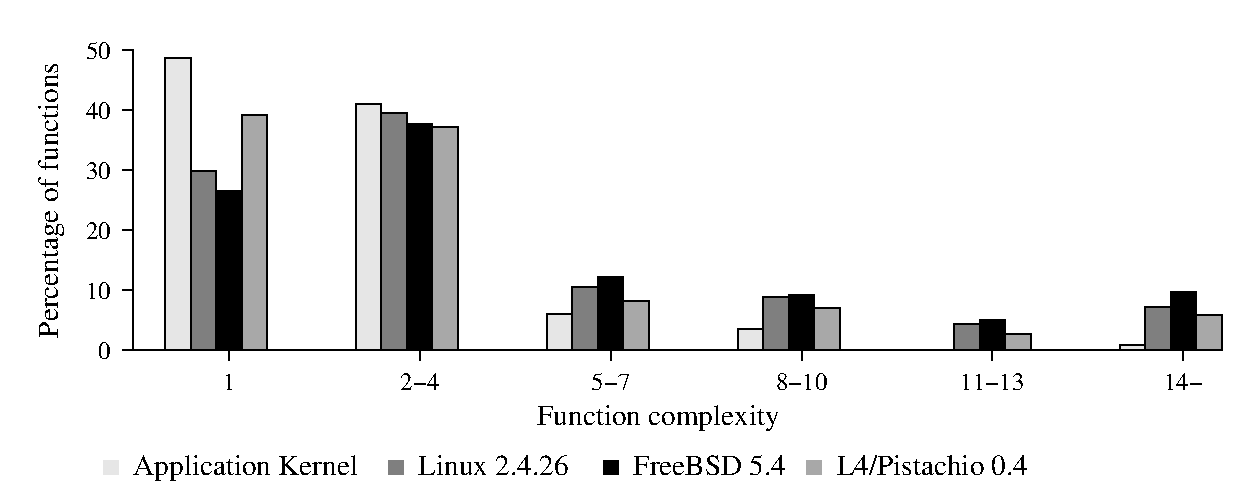
\epsfig{width=1.0\linewidth, file=./data/linux-appkern/mccabe_hist.parsed}
  \caption[Histogram of McCabe cyclomatic complexity]{Histogram of McCabe cyclomatic complexity for the Application
    Kernel, Linux 2.4.26, FreeBSD 5.4 and the L4/Pistachio 0.4 microkernel.}
  \label{fig:mccabe}
\end{figure}

\section{Conclusions and Future Work}
\label{sec:appkern:conclusion}

In this paper we have presented the application kernel, an alternative
approach for adding SMP support to a uniprocessor operating system. Our
approach has lower implementation complexity then traditional approaches,
often without changes to the original uniprocessor kernel, while at the same
time providing scalable performance. In this sense, the application kernel
approach can be seen as a modern revitalization of the master-slave approach.
There are also similarities with approaches used in distributed systems.

We have evaluated a prototype implementation of the application kernel
approach for a uniprocessor Linux kernel, where the results show that our
approach is a viable method to achieve good performance in computationally
intensive applications. We also show that the implementation is quite
straightforward, with a low cyclomatic complexity compared to other operating
system kernels and a small size (around 3,600 lines) requiring only seven
weeks to implement.

There are several advantages with our approach. First, we do not need to
modify the large and complex code of the uniprocessor kernel.  Second, the
development of the uniprocessor kernel can continue as usual with improvements
propagating automatically to the multiprocessor version. Our evaluation also
shows that a large portion of the effort of writing the application kernel can
be reused for other uniprocessor kernels which leads us to believe that our
approach and implementation is fairly generic and reusable for other kernels.

There are a number of optimizations possible for the application kernel
approach. For instance, some threads could run entirely on the bootstrap
kernel, which would mainly be interesting for kernel-bound applications. A
migration scheme similar to that in MOSIX could then be used to
move kernel-bound threads to the bootstrap processor during runtime. Further,
some system calls should be possible to implement directly on the application
kernel, providing the semantics of the system calls are known. For example,
sleeping, yielding the CPU and returning the process ID of the current process
can easily be implemented in the application kernel.

\section*{Acknowledgements}
We would like to thank the anonymous reviewers for their useful feedback. This
work was partly funded by The Knowledge Foundation in Sweden under a research
grant for the project ``Blekinge - Engineering Software Qualities (BESQ)''
(\url{http://www.ipd.bth.se/besq}).

\noindent
The application kernel source code is available as free software licensed
under the GNU GPL at
\url{http://www.ipd.bth.se/ska/application_kernel.html}.
